\documentclass{beamer}



%Information to be included in the title page:
\title{\textbf{Detecting changes in dispersion in COVID-19 case counts using a negative binomial model}}
\subtitle{JSM 2024}
\author{Rachael Aber, Yanming Di, Ben Dalziel}
\logo{
\includegraphics[height=1.1cm]{osu_logo}}

% import citation package
\usepackage[backend=biber]{biblatex}
\addbibresource{references.bib}

% font size package
\usepackage[font=footnotesize,labelfont=bf]{caption}

\AtBeginSection[]
{
	\begin{frame}
		\frametitle{Table of Contents}
		\tableofcontents[currentsection]
	\end{frame}
}

\begin{document}

\frame{\titlepage}

\begin{frame}
	\frametitle{Table of Contents}
	\tableofcontents
\end{frame}

\section{Why study variability?}
	
\begin{frame}
\frametitle{Why study variability?}
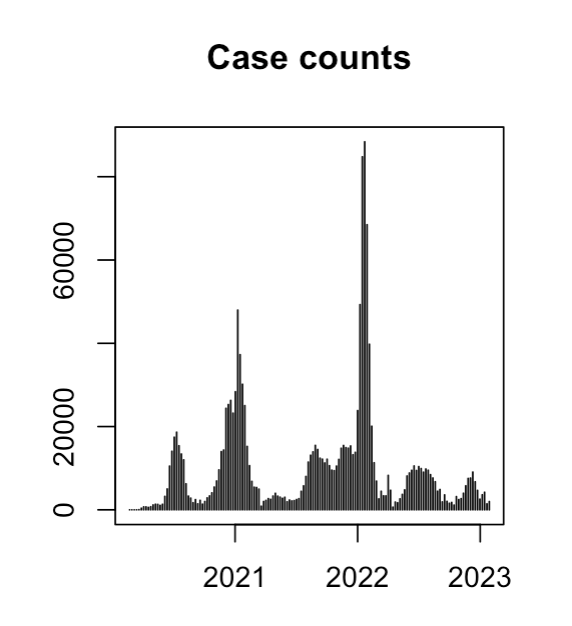
\includegraphics[height=4cm]{var}
\begin{itemize}[<+-| alert@+>] % other than alert it's also okay to insert \pause manually.
			\item Highly variable case count time series suggest transmission heterogeneity or changes in R
			\item Metrics of variability are overlooked: "How is variability related to different phases of an epidemic?"\cite{graham_measles_2019}
			\item Adam et al.\cite{adam_time-varying_2022} found that COVID-19 transmission heterogeneity decreased over time
	\end{itemize}
\end{frame}

\begin{frame}{\textbf{Why study variability?}}
	\begin{itemize}[<+-| alert@+>] 
		\item Dispersion of a case count time series may be a useful metric--part of a framework that models variance flexibly
		\item A 'mean crowding' parameter \cite{lloyd_mean_1967} was proposed: mean number per individual of other individuals in the same quadrat 
		\item Useful way to think about dispersion in case count time series, degree of dispersion is degree of clustering/crowding of cases (from the perspective)
		\item 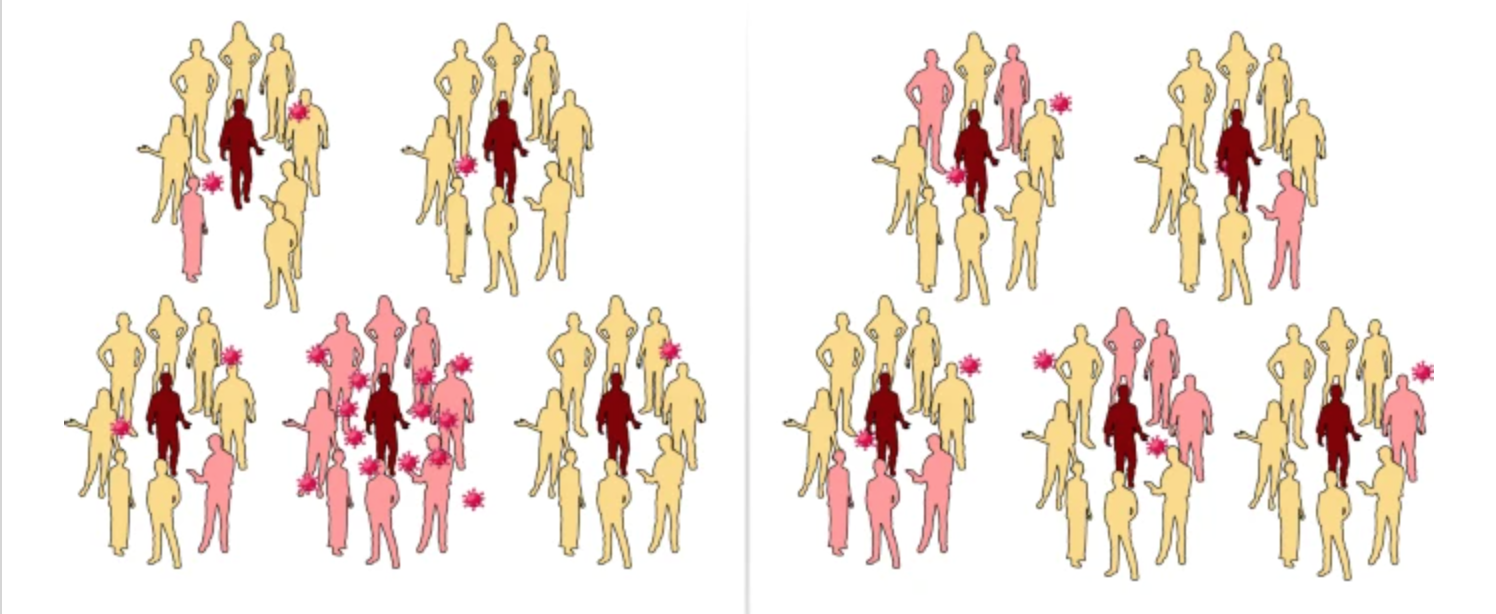
\includegraphics[height=2cm]{sup}
	\end{itemize}
\end{frame}

\section{Negative binomial model}
\begin{frame}{\textbf{Introduction to the method}}
	\begin{itemize}[<+-| alert@+>] 
		\item Let \begin{math}\lambda_t\end{math} be epidemic intensity, I\begin{math}_t\end{math} be incidence at time t, and \begin{math}\theta_t\end{math} be dispersion at time t
		\item \begin{equation}
			\mathrm{I_t = NB(\mu = \lambda_t, \theta_t = I_{t-1})} \cite{grenfell_dynamics_2002}
		\end{equation}
		\item Adjusted for population size using an offset in the model
		\item Linear predictor includes a natural spline in time to account for autocorrelation in case counts (ns are)
		\begin{align}
			log(E[Y_i]/n_i) &= \beta_1h_1(t_i) + \beta_2h_2(t_i) + \beta_3h_3(t_i) \\
			log(E[Y_i])-log(n_i) &= \beta_1h_1(t_i) + \beta_2h_2(t_i) + \beta_3h_3(t_i) \\ 
			log(E[Y_i]) &= \beta_1h_1(t_i) + \beta_2h_2(t_i) + \beta_3h_3(t_i) + log(n_i) 
		\end{align}
            \item Model fit on a rolling basis to each time series (one estimate)
	\end{itemize}
\end{frame}

\begin{frame}{\textbf{Negative binomial model}}
	\begin{itemize}[<+-| alert@+>] 
		\item 
            \begin{equation}
                f_t(I) = \binom{I + \theta - 1}{I} \left( \frac{\mu}{\mu+\theta} \right)^I \left( \frac{\theta}{\mu +\theta} \right)^\theta
            \end{equation}
		\item \begin{align}
		E(I) &= \mu\\
		Var(I) &= \mu + \frac{\mu^2}{\theta}
	\end{align}
	\item LRT framework: at each time step along a time series, fit null and full(\begin{math}\theta\end{math} change) model, conduct LRT to produce p-value at each time point
	\end{itemize}
\end{frame}

\begin{frame}{\textbf{Simulated time series data set}}
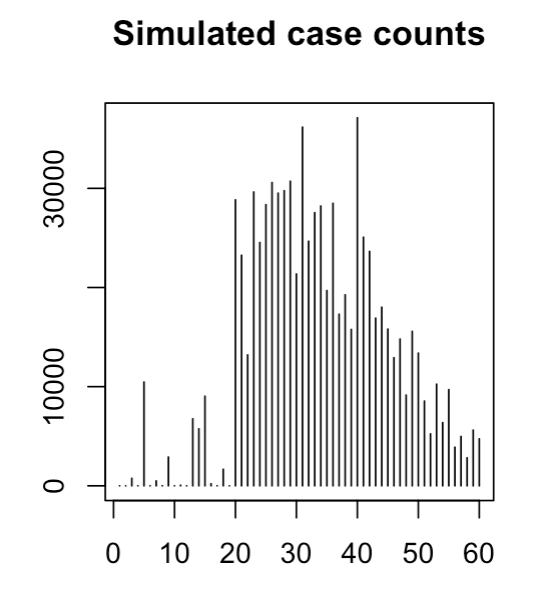
\includegraphics[height=3cm]{sim}
\begin{itemize}[<+-| alert@+>]
	\item Validity/power simulations: Gaussian and uniform epidemic curves with an attack rate of 0.1 
 	\item Varying magnitude of \begin{math}\theta\end{math} change, location of the change, underlying population size, and epidemic curve shape (allowed)
	\item Epidemic curves over 60 time steps each were produced, and the likelihood-ratio test (LRT) procedure was applied to each
\end{itemize}
\end{frame}

\begin{frame}{\textbf{Application to empirical data}}
	\begin{itemize}[<+-| alert@+>]
            \item Weekly case counts from US counties between 2020-01-04 and 2023-03-18
		\item Estimated \begin{math}\theta_t\end{math} for 154 time steps for 144 US counties (IRLS procedure implemented via the NBPSeq package\cite{NBPSeq} and from Di et al.\cite{yanming_nbp_2011}) 
		\item We investigated large counties (largest three counties in each state)
	\end{itemize}
\end{frame}

\section{Results}
\begin{frame}{\textbf{Results: simulated data}}
	\begin{itemize}[<+-| alert@+>]
		\item Negative binomial/LRT method is robust to differences in population size (for population sizes examined)
		\item Illustrated that an increase in \begin{math}\theta\end{math} is associated with decreased variability in simulated incidence time series  (same relationship is observable in the empirical time series), with an increase in \begin{math}\theta\end{math} corresponding to a decrease in variability around the trend in incidence
	\end{itemize}
\end{frame}

\begin{frame}{\textbf{Results: simulated data}}
		\begin{figure}[!h]
			
\includegraphics[width=0.6\textwidth]{fig1}
			\caption{
				Detecting dispersion changes in incidence time series in populations of different sizes. A/B: Simulated incidence when dispersion is constant/changes. C/D: Constant/changing dispersion used in generation of above. E: Performance of LRT with simulated data that has different absolute differences in theta (horizontal axis of each pane) illustrates p-value distribution across different population sizes (each pane is one population size). O and X mark the null and alternative hypotheses indicated in panels C and D. 
			}
			\label{fig1}
		\end{figure}
\end{frame}

\begin{frame}{\textbf{}}
		\begin{figure}[!h]
			
\includegraphics[width=0.6\textwidth]{compare}
			\caption{
				Method applied to case counts between 2020-01-04 and 2023-03-18 for Jefferson County, AL. A: Case counts . B: LRT statistic C: Log dispersion parameter.
			}
			\label{fig2}
		\end{figure}
\end{frame}

\begin{frame}{\textbf{Results: empirical data}}
	\begin{itemize}[<+-| alert@+>]
		\item Highly overdispersed incidence observed more frequently later in time series (consistent) (Most dispersed category in Fig reaches) 
		\item Evidence for a change in \begin{math}\theta\end{math} was observed across many counties (evidenced by concentration of low p-values around peak incidence) 
		\item High dispersion may indicate less diffuse epidemics that are potentially more subject to climate forcing\cite{dalziel_urbanization_2018}, or increased locally experienced mean density \cite{lloyd_mean_1967}
            \item Raising variance relative to mean implies spatiotemporal "crowding" of cases (i.e. localized surges) which may necessitate more surge capacity in hospitals and testing centers

	\end{itemize}
\end{frame}

\begin{frame}{\textbf{Results: empirical data}}
	\begin{figure}[!h]
	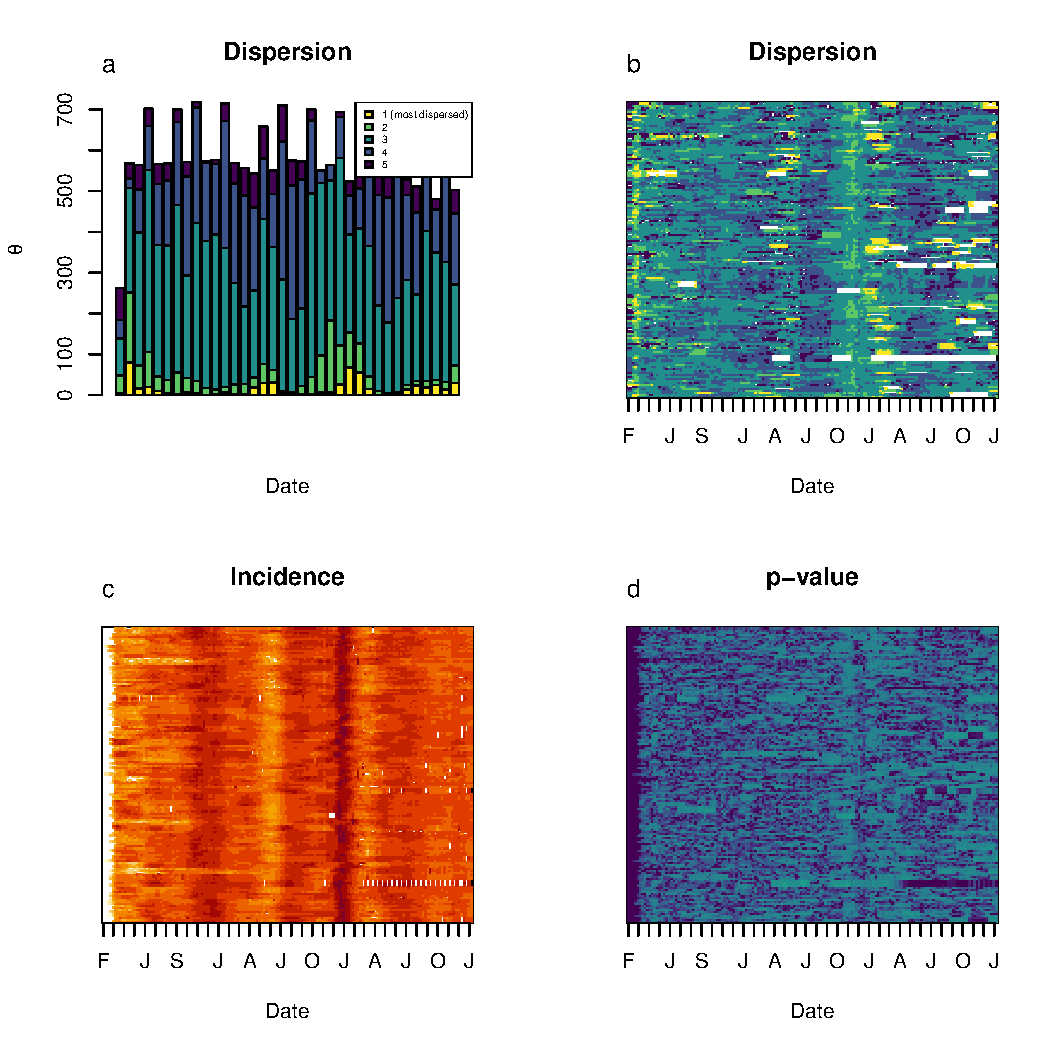
\includegraphics[width=0.6\textwidth]{fig2}
	\caption{
		Incidence and dispersion in large counties in the US. A: Binned log of the dispersion parameter. B: Log of the dispersion parameter for each of the large counties (y-axis). C: Log incidence for each of the large counties (y-axis). D: LRT p-values for each of the large counties (y-axis).
	}
	\label{fig2}
\end{figure}
\end{frame}

\section{Concluding remarks}
\begin{frame}{\textbf{Concluding remarks}}
	\begin{itemize}[<+-| alert@+>]
            \item LRT procedure performs well for relevant range of population sizes
            \item Dispersion parameter and LRT statistic don't simply reflect changes in process mean
		\item Dispersion is high at unexpected times (near peak incidence)(changes)
            \item Methods that use time series are crucial (due to); timing/allocation of public health resources can be achieved (with, pop less effective) 
	\end{itemize}
\end{frame}

\section{References}

\begin{frame}
    \printbibliography
\end{frame}

\begin{frame}
	\begin{center}
		{\Huge Thanks!}
	\end{center}
\end{frame}

\end{document}